\chapter{Search Strategy}
\label{ch:SearchStrategy}

We will reconstruct many different physics objects, interesting particle tagging methods or kinematic variables unique to the collisions. There are many different types of particles that we are interested in when working with particle physics measurements. These particles have very short lifetimes $\tau_t\approx10^{-25}$ s for the $t$ quark \cite{quadt_top_2007} and $\tau_b\approx10^{-12}$ s for the $b$ quark \cite{lenz_lifetimes_2019}. We are interested in certain physics objects such as jets (\nj), Heavy object tagging (\nb, \nt, \nrt, \nw), missing transverse momentum (\met), soft-b tagging (\nsv), Initial State Radiation, and lepton identification. We will look into each of these objects further in this chapter.

 %We mainly interact with the decay products of the event, such as, jets $(N_j)$, heavy object tagging $(\nb, \nt, \nw, \nrt)$, missing transverse momentum (\met), scalar sum jet momentum $(H_T)$, soft-b tagging, denoted as $\nsv$, transverse mass between tagged $b$ quarks and \met{} $(m_T(b_{1,2}, \met))$, Initial State Radiation, and lepton identification. We will look into each of these objects further in this chapter.
 
 \section{Physics Objects}\label{PhysObj}
 We will discuss each of the physics objects that we need to design the search region for our analysis. These can be basic objects such as, jet reconstruction of missing transverse momentum, or high level objects such as, transverse energy and heavy object tagging.

\subsection{Jets}\label{Jets}
In an interaction, whenever a quark is produced, it comes in pairs $(q\overline{q})$. When a quark pair is produced they form a color flux tube. As they quickly start to move away from each other, in the center-of-momentum frame, the energy density of the color flux tube will increase to the point that another $q\overline{q}$ pair can be produced. This will continue to occur in a sequence of radiating gluons or photons and the production of pairs of particles, see Fig. \ref{JetHadronization}. 
In the detector, the energy deposited in the HCAL is a cluster of charged or neutral particles of a radius, $\Delta R=\sqrt{\Delta\eta^2+\Delta\phi^2}$. There are many algorithms to reconstruct the jets which must satisfy the requirements in Ref. \cite{noauthor_jet_2010}. We are mainly interested in the \antikt{} Jet algorithm \cite{cacciari_anti-ktjet_2008} method which uses the transverse momentum of the particles within a certain radius $\Delta R = 0.4 (0.8)$ for AK4(AK8) jets \cite{noauthor_https://twiki.cern.ch/twiki/bin/view/cms/jetid_nodate, noauthor_https://twiki.cern.ch/twiki/bin/view/cms/introtojec_nodate}. 

The measurement of interest is the distance $d_{ij}$ between the particles $(i)$ and pseudojets $(j)$ and $d_{iB}$ as the distance between the particle and the beam $(B)$. The clustering identifies the smallest distance and if it is $d_{ij}$ the particle is added to the pseudojet, while if it is the distance $d_{iB}$ it is classified as a jet and removed from consideration. The distances are recalculated and repeated for all particles, see Fig. \ref{antikTJetReco}. The generalized algorithm is defined by the following distance measurement,
\begin{equation}\label{eqn:antikT}
\begin{split}
d_{ij}&=\text{min}(k_{ti}^{2p},k_{tj}^{2p})\frac{\Delta^2_{ij}}{R^2} \\
d_{iB}&=k_{ti}^{2p} \\
\end{split},
\end{equation}
where $\Delta^2_{ij}=(y_i-y_j)^2+(\phi_i-\phi_j)^2$, $k_{ti}$ is the transverse momentum, $y_i$ is the rapidity, $\phi_i$ is the azimuthal angle, and $R$ is the radius parameter of the pseudojet. The above becomes the \antikt{} algorithm when $p=-1$. The jet area of the reconstructed jets are circular since the \antikt{} jets are unaffected by soft radiation. It is also insensitive to pileup which is of particular importance in CMS. An additional feature is that it is infrared safe, such that soft emissions of particles will not effect the reconstructed jets. 

A charged hadron subtraction is also used to correct for the pileup, the number of collisions seen during a single proton beam crossing \cite{cacciari_pileup_2008, noauthor_pileup_2014}. For AK8 jets the pileup contribution is accounted for using the "pileup per particle identification" method \cite{bertolini_pileup_2014, noauthor_pileup_2014}, where each particle is weighted by its probability of originating from the primary vertex. Once the jets have been identified, we can analyze their respective properties to determine the likelihood of the particle it originated from, such as a $b, t,$ or \W. 

\begin{figure}
 	\centering
	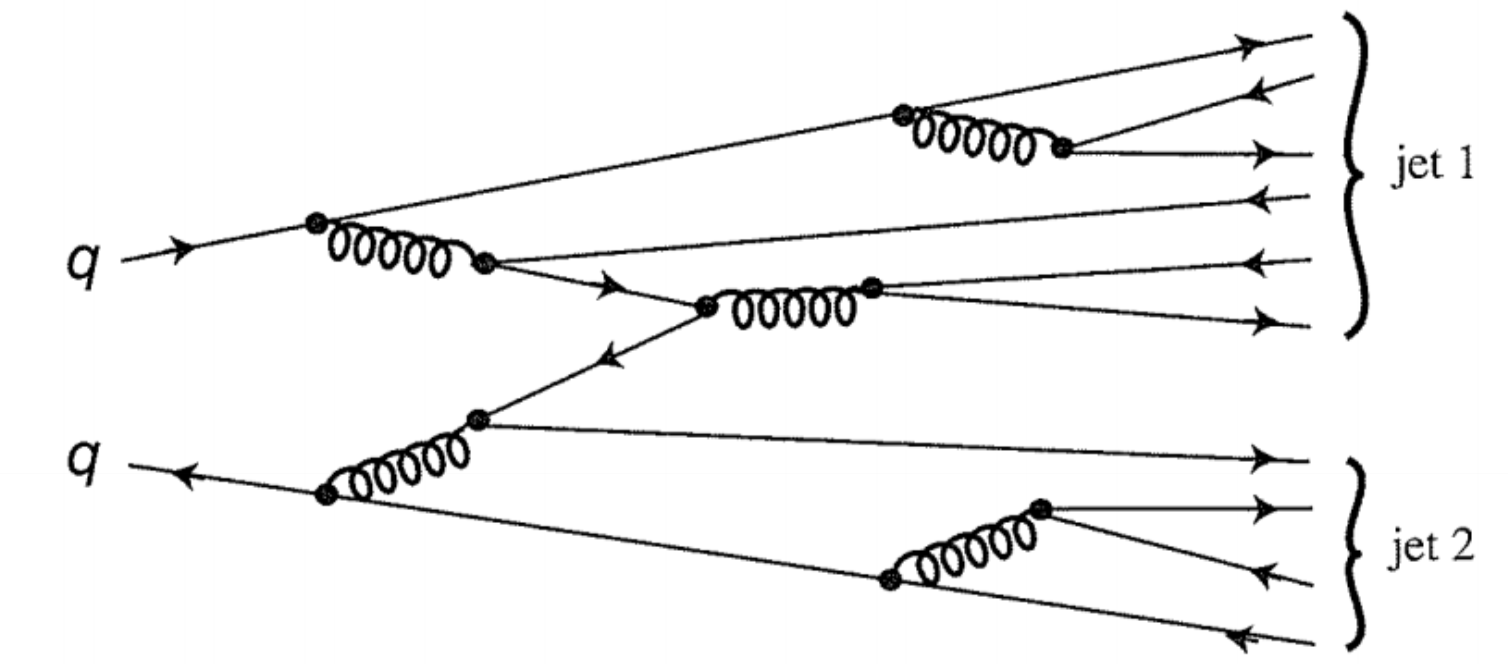
\includegraphics[width=0.75\textwidth]{JetHadronization.png}
 	\caption[Jet Hadronization]{A diagram of a quark pair radiating gluons that decay into more quark pairs in a process called hadronization \cite{griffiths_introduction_2008}.}
 	\label{JetHadronization} 
\end{figure}

\begin{figure}
 	\centering
	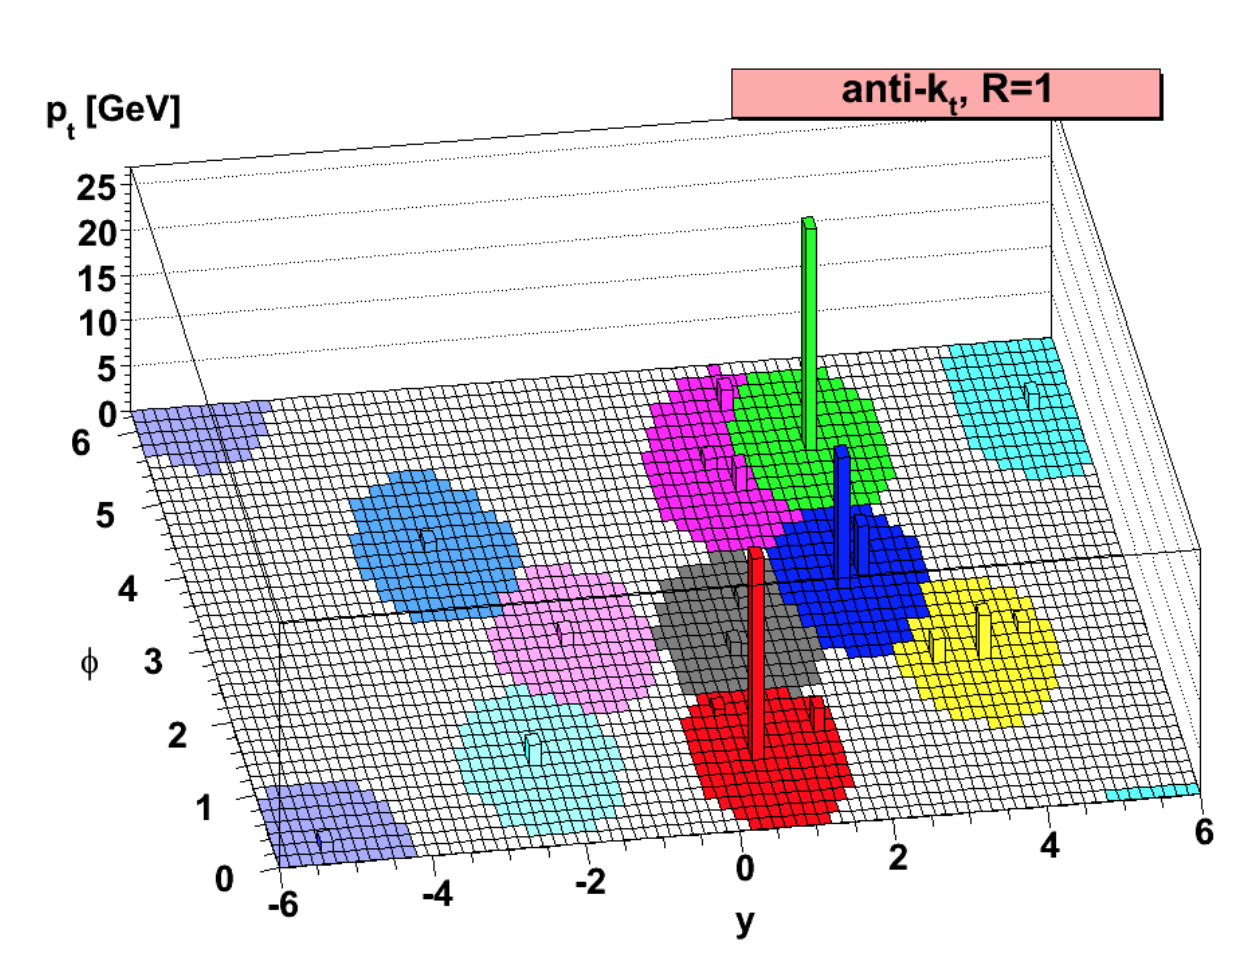
\includegraphics[width=0.75\textwidth]{antikT_jetReconstruction.png}
 	\caption[Anti-$k_T$ Jet Reconstruction]{A sample parton level event with random soft particles that is clustered with the anti-kT algorithm \cite{cacciari_anti-ktjet_2008}.}
 	\label{antikTJetReco} 
\end{figure}

\subsection{Heavy Object Tagging}\label{HeavyObject}
Since this search is looking for a massive particle which then decays to slightly less massive particles we need to be able to identify and distinguish between them. We use various algorithms and neural networks to identify jets from $b$ quarks, $t$ quarks, or from \W {} bosons. 

\subsubsection{B-Tagging}\label{Btagging}
The ability to identify secondary vertices is essential in searches for the top squark, see Sec. \ref{sec:Production}. Since the b quark is a long lived particle, about $10^{-12}$ seconds, it will travel many millimeters before decaying into other particles. A \B{} quark is identified during reconstruction, where the jet originating from a point separated from the primary vertex $(PV)$, known as the secondary vertex $(SV)$. The displaced vertex of the long lived $b$ quark with low \pt{} has many interesting kinematic properties that we can use to identify them, $b$-tagging. 

Now \B-tagged jets are jets that are likely to have originated from a \B{} quark. For \B{} quarks with large transverse momentum, we use a Deep Combined Secondary Vertex (DeepCSV) algorithm that involves neural networks\cite{noauthor_performance_nodate}. The medium working point recommended by the B-tag Physics Object Group (POG), corresponding to a threshold of 0.6324 0.4941, and 0.4184 for the 2016, 2017, and 2018 eras, respectively \cite{noauthor_https://twiki.cern.ch/twiki/bin/viewauth/cms/btagrecommendation2016legacy_nodate, noauthor_https://twiki.cern.ch/twiki/bin/viewauth/cms/btagrecommendation94x_nodate, noauthor_https://twiki.cern.ch/twiki/bin/viewauth/cms/btagrecommendation102x_nodate, noauthor_https://twiki.cern.ch/twiki/bin/viewauth/cms/btagsfmethods_nodate}. The medium working point is defined such that the percentage of a light jet being misidentified as a $b$ jet is 1\%.

\begin{figure}
 	\centering
	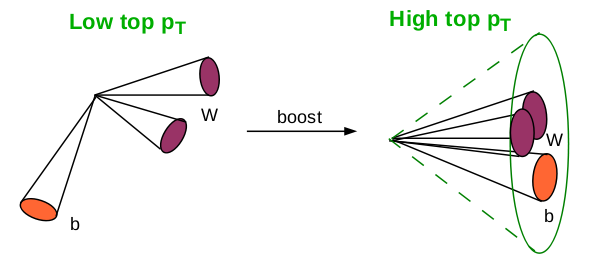
\includegraphics[width=0.75\textwidth]{TopDecayBoost.png}
 	\caption[Top Decays]{The two types of top quark reconstructions, when each decay product is easily identifiable (resolved) or when the particles are close together (boosted).}
 	\label{TopDecays} 
\end{figure}

\subsubsection{Top/W Tagging}\label{TopTagging}
Top quark tagging is an essential part of our analysis. The top quark tagging algorithm is designed to have a high reconstruction efficiency for entire \pt{} spectrum of the top quark in our signal models. The \antikt{} algorithm using a distance parameter, $\Delta R=0.8$, is expected to contain the energy clusters of all of the decay product of boosted $t$ quarks \cite{noauthor_top_nodate, aad_identification_2016}, see Fig. \ref{TopDecays}, with $\pt>300$ GeV or \W{} bosons with $\pt>200$ GeV. These decays are reminiscent of the expected decay, $t\rightarrow bq\bar{q}^\prime$, when it is a highly Lorentz boosted $t$ quark decay. The requirements are:
\begin{itemize}
	\item Medium working point $>0.937, 0.895, 0.895 (0.973, 0.991, 0.991)$ for boosted $t$ $(W)$ for the separate 2016, 2017, and 2018 eras, respectively \cite{ganin_unsupervised_2015}.
	\item Reconstructed soft drop\cite{larkoski_soft_2014, dasgupta_towards_2013} mass: $105<m_t<210$ GeV and $65<m_W<105$ GeV.
	\item Boosted tops: $\pt=300$ GeV, $|\eta|<2.0$ and $W$: $\pt=200$ GeV, $|\eta|<2.0$.
\end{itemize}

There is another type of top that can be reconstructed, which is when each subjet of the top decay can be resolved into each individual jet, denoted as a resolved top \cite{ganin_unsupervised_2015}, see Fig. \ref{TopDecays}. The requirements are:
\begin{itemize}
	\item Medium working point: 0.92 for all eras.
	\item $|\eta(j_{1,2,3})|<2.4$ and $b$-tag discriminator: $>0.6324, 0.4941, 0.4184$ for the separate 2016, 2017, and 2018 eras, respectively. The number of jets in the event that pass these cuts should be $\geq2$.
\end{itemize}
These object definitions, \nt, \nw, \nrt, are chosen such that there is no overlap in their definitions and are used to bin our search and control regions. 

\subsection{Missing Transverse Momentum}\label{MET}
The missing transverse momentum \cite{lester_measuring_1999, barr_variable_2003} is the negative vector sum of the total transverse momentum measured in the detector,
\begin{equation}
\met=-\sum_{i\in\text{vis}}\overrightarrow{p}_{i, T},
\end{equation}
where the sum of the momentum runs over every visible (vis) particle in the event \cite{collaboration_missing_2011,penning_pursuit_2018}. We use the transverse component of the momentum because the $z$ component of the particle momentum is not exactly known. We know the center-of-momentum for the system but cannot know how each proton is boosted. Since the $x$ and $y$ components are orthogonal to the direction of the boost they are unaffected by the boost of each individual interaction. Ideally, if the detector was $100\%$ efficient this quantity would always be zero due to conservation of momentum, but many things, such as detector efficiency, particle misidentification, or particles that are weakly interacting such as neutrinos or \neutralino. Because of these, \met{} is a good discriminator for searching for physics beyond the SM \cite{noauthor_https://twiki.cern.ch/twiki/bin/view/cms/missingetrun2corrections_nodate}. 

%\subsection{MET Filters}
%Need to add MET Filters here.

\subsection{$H_T$}\label{HT}
Another interesting quantity is \Ht, which is the scalar sum of the \pt{} of all of the jets in an event \cite{cms_collaboration_search_2011},
\begin{equation}
\Ht=\sum_{i\in\text{jets}}p_{i,T}.
\end{equation}
This quantity is quite useful when trying to identify massive particles and is quite good at suppressing QCD multijet background. Since \Ht{} is a sum of all jets, it is specifically good at identifying particles that are massive and produce jets that can be measured in the CMS calorimeters. For QCD events that mainly contain quark(gluon) jets that are not $t$ tend to not have as much energy as such that the \Ht{} is small. 

\subsection{Soft $b$-Tagging}\label{SV} 

\begin{figure}
 	\centering
	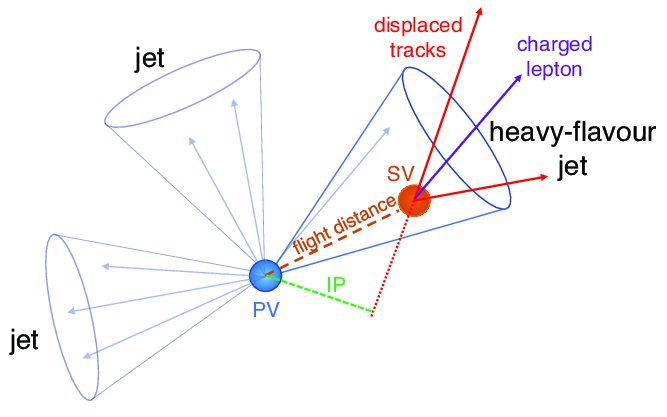
\includegraphics[width=0.75\textwidth]{SecondaryVertex.png}
 	\caption[Secondary Vertex Diagram]{An interaction that produces a long lived particle that has a reconstructed SV.}
 	\label{SecondaryVertex} 
\end{figure}

Soft $b$-tagging is used for $b$ quarks that have low \pt. This search also targets models that produce very soft (low \pt) bottom or charm quarks. A large fraction of events contain b quarks with \pt{} below the 20 GeV jet threshold which may fail to be reconstructed as jets or become b-tagged due to either the SUSY mass spectrum or kinematics causing a large boost along the beam line. Identification of these soft quarks improves our ability to separate potential signal events from the SM background. We therefore aim to identify $b$ or $c$ quarks based on the presence of a SV reconstructed using the Inclusive Vertex Finder (IVF) \cite{noauthor_https://twiki.cern.ch/twiki/bin/view/main/inclusivesecondaryvertexfinder_nodate, fruehwirth_new_2003}. Additional requirements on the SV observable are applied to suppress the background originating from light quarks. These selected SV may be referred to as soft $b$-tags and are constructed to be an addition to the jets and b-tagged jets used in this analysis to improve efficiency. 

The requirements on each SV to pass the soft b-tagging definition are:
\begin{itemize}
	 \item The distance in the transverse plane between the SV and the PV $\leq3$ cm.
	 \item The significance of the distance between the SV and the PV in 3D, $\sigma_{IP}^{3D}\geq4$.
	 \item The pointing angle, defined as $\cos(\overrightarrow{PV,SV},\overrightarrow{p_{SV}})\geq0.98$, where $\overrightarrow{PV,SV}$ is the vector pointing from $PV$ to $SV$ and $\overrightarrow{p_{SV}}$ is the total four-momentum of the tracks associated with the SV. 
	 \item The number of tracks associated with the SV is greater or equal to 3.
	 \item The \pt{} of the particles associated SV is less than 20 GeV.
\end{itemize}
Identification of soft b-quarks is necessary for a potential signal region where the stop does not directly decay into a top quark and is essential for some of our search region bins. 

\subsection{Initial-state Radiation}\label{ISRpt}

Initial-state radiation (ISR) may be clustered into one of the large-$R$ jets clustered with a distance parameter, $\Delta R=0.8$. We use the larger radius jets to be sensitive to ISR with gluon splitting, when a jet radiates a gluon that pair produces two quarks. The ISR jet is identified as being the hardest of the large-$R$ jets with $\pt>200$ GeV which fails the loose b-tagging working point and is not identified as a top or W. This is a good parameter for jets that are neither tagged as $t$ or \W{} in the low \dm{} region of our search.
 
\subsection{Electron and Muon Identification}\label{EleMuonID}
 This is a search for all-hadronic decays so no leptons are expected in the search region, however, for some control regions we require exactly one lepton so an efficient tagging method is necessary. There are two sets of selection criteria used in the analysis for electrons \cite{noauthor_performance_2015} and muons \cite{collaboration_performance_2013, cms_collaboration_performance_2018}. The set of criteria used to efficiently reject events with an isolated electron is done with a "Veto" ID. An electron with a Veto ID must pass the following cuts for the barrel (endcap) regions of the detector:
 \begin{itemize}
	 \item $|\Delta\eta|<0.007(0.01),|\Delta\phi|<0.8(0.7)$ for the EM showers in the ECAL,
	 \item $\sigma_{i\eta i\eta}=\frac{\sum(\eta_i-\overline{\eta})^2w_i}{\sum w_i}<0.01(0.03)$ where $\overline{\eta}=\frac{\sum\eta_iw_i}{\sum w_i}$ and $w_i=\text{max}(0,4.7+log(E_i/E_{5\times5}))$ where the sum is over a $5\times5$ crystal matrix centered arount the most energetic crystal in the ECAL \cite{collaboration_missing_2011},
	 \item $H/E<0.15$ (not applicable) the ratio of hadronic energy over electromagnetic energy,
	 \item $\text{PF isolation}/\pt(\Delta R=0.3)<0.15(0.15)$ where we are calculating the \pt{} of the various energy deposits (charged hadrons, photons, and neutral hadrons) as the \pt{} for the PF Isolation and dividing it by the sum of the \pt{} of the listed candidates in a cone with a size of $\Delta R=0.3$,
	 \item $|d_{0}|<0.04(0.04),|d_z|<0.2(0.2)$ where $d_0$ is the distance in the $xy$ plane and $d_z$ is the distance along the $z$-axis for the reconstructed candidate.
 \end{itemize}
This veto ID is chosen such that the search region is most likely to be devoid of electrons, since it has a 95\% efficiency \cite{noauthor_https://twiki.cern.ch/twiki/bin/view/cms/cutbasedelectronidentificationrun2_nodate}.
 
 We use the Loose muon definition recommended by the Muon POG for the purposes of the muon veto \cite{noauthor_https://twiki.cern.ch/twiki/bin/view/cmspublic/swguidemuonidloose_muon_nodate}. A Loose muon is identified as a Particle Flow (PF)\cite{noauthor_cms_nodate} muon and can be either a global muon or an arbitrated tracker muon. Only candidates with transverse (longitudinal) impact parameter $|d_0|<0.2$ cm $(|d_z|<0.5 \text{cm},)$ with respect to the primary vertex, are considered. The electron and muon IDs are used in the definition of the Lost Lepton background which will be expanded upon further in Section \ref{sec:LL}. 
 
\subsection{Tau Identification}\label{TauID}
Identification of taus, which is a long lived particle $\tau_\tau=2.9\times10^{-13}$ s, is necessary in an all-hadronic analysis, but a tau has the possibility of decaying hadronically, $\tau^+\rightarrow \pi^+\pi^0\overline{\nu}_\tau$. The tau can decay both leptonically and hadronically with $\approx17\%$ of decays to electrons or muons each, $\approx51\%$ of decays to $1$ hadron with $\geq1$ neutral hadrons, and $\approx15\%$ for 3 hadrons with $\geq1$ neutral hadrons. The tau decays that are leptonic should be identified by the muon or electron IDs, but the hadronic decays are a bit more difficult. We are using a combined isolated track (IsoTrack) and MVA method for identifying a hadronically decaying tau. 

The IsoTrack requirements are:
\begin{itemize}
	\item pdgId = 11 or 13 (211) where pdgId is the particle data group Id from the reconstructed particle and 11 = electron, 13 = muon, and 211 = pion,
	\item $\pt\geq5(10)$ GeV and $iso>0.2(0.1)$ for electrons and muons (pions) where the isolation is the separation from other particle for a cone of $\Delta R=0.2$,
	\item $m_T(l,\met)\leq100$ GeV is the transverse mass between the candidate lepton and \met, see Sec. \ref{sec:transverseMass}
\end{itemize}

The Tau ID has been studied extensively in tests which looked into the custom multivariate analysis (MVA) \cite{roe_boosted_2004, hoecker_tmva_2007, bravo_search_2015} similar to the one used in Ref. \cite{cms_collaboration_search_2016}, a cut-based IsoTrack method, and Tau POG MVA method of identifying hadronically decaying taus. The methods which provide the best improvement to the efficiency of identifying taus with a small fake rate is the combination of IsoTrack and Tau POG MVA. With the inclusion of the combined method for identifying hadronically decaying taus, the veto percentage is $\frac{N_\tau>0}{N_{gen}>0}\approx29.0\%(7.2\%)$ with an efficiency of the veto of $\frac{N_\tau>0\text{ \& }N_\tau^{gen}>0}{N_\tau^{gen}=0}\approx49.1\%(22.6\%)$ for \ttbar{} background (signal), see Appendix. \ref{sec:TauMVA}. 

For the IsoTrack method we require the following:
\begin{itemize}
	\item $\pt\geq5(10) \text{GeV}, \text{iso}\leq0.2(0.1)$ for electrons and muons(pions);
	\item $m_T(\text{IsoTrack},\met)<100$ GeV;
\end{itemize}
where $m_T(\text{IsoTrack},\met)$ is the transverse mass between the IsoTrack and \met. For the Tau POG method we require:
\begin{itemize}
	\item $\pt\geq20 \text{GeV}, |\eta|<2.4$;
	\item Decay mode $=5(N_c-1)+N_p\geq0$ where $N_c$ is the number of charged hadrons and $N_p$ is the number of pions in the decay it is a descriminator developed to identify taus decaying to multiple prong events; and
	\item Medium working point.
\end{itemize}
With the inclusion of the separate electron/muon IDs and the combined IsoTrack + TauPOG IDs we have a method to efficiently veto leptons from our search region.

\subsection{Transverse Energy between $b$ quarks and \met} \label{sec:transverseMass}
We will end up dividing the search regions we are interested in into two different groups. They will be distinguished by a parameter known as the transverse mass between the leading \bjet{} and \met{} defined as:
\begin{equation}\label{TransverseMass}
M_T(b,\met)=\sqrt{2\cdot\met\cdot\pt(b)(1-\cos(\Delta\phi(\met,\pt(b))))},
\end{equation}
where $\Delta\phi(\met,\pt(b))$ is the angle, $\phi$, between \met and the leading $b$ jet, $(p(b))$. A feature of $M_T(b,\met)$ when used for a parent particle that decays to a visible and invisible particles, such as $\W^+\rightarrow l^+\nu_l$ will have a peak at the \W{} mass in the rest frame \cite{tovey_transformation_2019}.This will be used to distinguish between our low and high mass search regions, see Section \ref{SearchRegions}.

\section{Samples and Filters}\label{Samples}
A detailed list of the samples and filters used in this analysis are described in Appendix \ref{sec:SamplesApp}.

\section{Baseline Selection} \label{sec:Baseline}

Following the same methods as above, we have a loose pre-selection which is referred to as the baseline selection. This will place a selection on jets and \met, which is used to eliminate a large fraction of background events. We define the baseline selection as:
\begin{itemize}
	\item $N_{e,\mu} = 0, (\pt\geq5$ \GeV, $|\eta|<2.5(2.4), \text{miniISO}<0.1(0.2))$ where the ISO is the sum of the \pt{} for the isolated tracks and calorimeter measurements divided by the lepton \pt;
	\item $N_{e/\mu/\pi}^{\text{trk}} = 0, (\pt\geq5 (10)$ \GeV, ISO $< 0.2(0.1) \text{ for electron/muons(pions)})$;
	\item $N_\tau = 0, (\pt\geq20$ \GeV, $|\eta|<2.4)$, medium working point;
	\item $N_{j} \geq 2, (\pt\geq30$ \GeV, $|\eta|<2.4)$;
	\item $\met\geq250$ \GeV, to reach the plateau of the trigger efficiency;
	\item $\Ht\geq300$ \GeV; and
	\item HEM Veto for part of 2018 data: $-3\leq\eta\leq-1.4, -1.57\leq\phi\leq-0.87$.
\end{itemize}
The HEM Veto is required due to a failure of two sectors of the HCAL endcaps on June 30th, 2018 which ended with the modules becoming unresponsive. These modules correspond to a region of $-3\leq\eta\leq-1.4, -1.57\leq\phi\leq-0.87$ which effect the lepton, jet, and \met{} reconstructions. This is applied to data from 2018 after Run 319077 and to the corresponding simulated events.
In addition to this, we allow for two separate sets of additional selections to apply to the low and high \dm{} search regions to further reduce background where the $\Delta m=m_{\st}-m_{\neutralino}$, see Fig. \ref{StopParameterSpace}. The high \dm{} baseline selection includes the baseline selection and additionally:
\begin{itemize}
	\item $N_j\geq 5, (\pt \geq30$ \GeV, $|\eta|<2.4)$;
	\item $N_b\geq 1, (\pt\geq20$ \GeV, $|\eta|<2.4)$, medium DeepCSV working point;
	\item $\text{Min}[|\Delta\phi(\met,j_1)|,|\Delta\phi(\met,j_2)|,|\Delta\phi(\met,j_3)|,|\Delta\phi(\met,j_4)|]\equiv\highdm$, where $j_1, j_2, j_3, j_4$ are the four leading jets in $p_T$. This requirement is to reduce the QCD multijet background since QCD events with \met{} are typically due to mis-measurement of the quark-gluon jets. 
\end{itemize}
Next, the low \dm{} baseline selection has the following addition selections:
\begin{itemize}
	\item $N_t=0, N_W=0,N_{res}=0,$ where $N_t$ and $N_W$ are the number of merged tops and \W's, respectively, and $N_{res}$ is the number of resolved tops;
	\item An ISR jet as defined in Sec. \ref{ISRpt} with $\pt(\text{ISR})\geq200$ GeV, $|\eta|<2.4, |\Delta\phi(j_{\text{ISR}},\met)|\geq2.$;
	\item $\met/\sqrt{H_{T}}\equiv S_{\met}\geq10$, where $H_T$ is calculated as the scalar sum of the \pt{} of jets with $\pt\geq30$ \GeV{} and $|\eta|<2.4.$; and
	\item \lowdm, where $j_1,j_2,j_3$ are the three leading jets in \pt. 
\end{itemize}

\subsection{Search Regions}\label{SearchRegions}

After applying the baseline selection criteria, we categorize events in the search sample into exclusive search regions that exploit the kinematic properties of different signal topologies, see \cite{cms_collaboration_search_2016, alwall_simplified_2009, alwall_model-independent_2009}. The search regions will be binned using the physics objects and kinematics variables explained above, such as, \nj, \nb, \nt, \nrt, \nw, \met, \Ht, \nsv, \mtb, and $N_{lep}=0$

For the search regions that mainly target high \dm{} signal models, we define two event categories in \mtb, see Section \ref{TransverseMass}, and a variable defined as:
\begin{equation}
\mtb\equiv
\begin{cases}
\begin{split}
& m_T(b,\met), &\nb=1 \\
& \text{Min}[m_T(b_1, \met),m_T(b_2,\met)], &\nb\geq2 \\
\end{split}
\end{cases},
\end{equation}
where $b_1, b_2$ are the two selected b-tagged jets with the highest values of the DeepCSV discriminator. In \ttbar{} events where the \W{} bosons decays leptonically and is missed by the lepton tagging, which is known as Lost Lepton background, the \mtb of such an event has a kinematic endpoint at the mass of the top quark, $m_t$.

We therefore define two event categories: $\mtb>175$ GeV and $< 175$ GeV, see Fig. \ref{StopParameterSpace}. In the low-\mtb{} category, to target signal models with moderate values of \dm, we define search regions by requiring $\nj\geq7$ and $\nrt\geq1$ to benefit from potential ISR in signal events while suppressing the SM background. Events are then subdivided according to the number of b-tagged jets $(\nb=1,=2,\geq3)$ and different \met{} thresholds. The same subdivision is performed for events in the high-\mtb{} category with $\nj\geq7$, but containing no top- or W-tagged candidates. We then target signal models with sufficiently boosted top quarks or W bosons by defining categories in the high-\mtb{} region that require the presence of at least one top- or W-tagged candidate. These categories do not have any further \nj{} requirement beyond that of the high \dm{} baseline selection, and are further subdivided according to $\nb, \met, \Ht$ and the number of each kind of top- and W-tagged candidate. Table \ref{tab:searchregions-hm} summarizes the definitions of all 130 disjoint search regions targeting high \dm{} signal models.

Events originating from low \dm{} signal models are likely to have lower values of \mtb \cite{sirunyan_search_2017}. We therefore only use the low-\mtb{} category to define search regions targeting these signal models. These search regions are further defined by the number of b-tagged jets, the number of identified secondary vertices (\nsv), the ISR jet \pt{} (\ptb), and \met. Events in the $\nb=0$ category, which targets very compressed signal models, are further subdivided according to \nj. Only events with very high ISR $\pt(>500~\GeV)$ are selected in this category, which is also categorized by the presence or absence of soft b-tagged secondary vertices. Events in the $\nb=1$ category are further characterized according to the \pt{} of the b-tagged jet into two sub-categories, while those in the $\nb\geq2$ are subdivided based on \ptbonetwo{} into three sub-categories, in order to take advantage of the softer b jet \pt{} spectrum expected in signal events compared to the SM background. Orthogonality to the high \dm{} event categories is achieved mostly by the \mtb{} categorization. Table \ref{tab:searchregions-lm}  summarizes the definitions of the 53 disjoint search regions targeting low \dm{} signal models.

\begin{figure}
 	\centering
	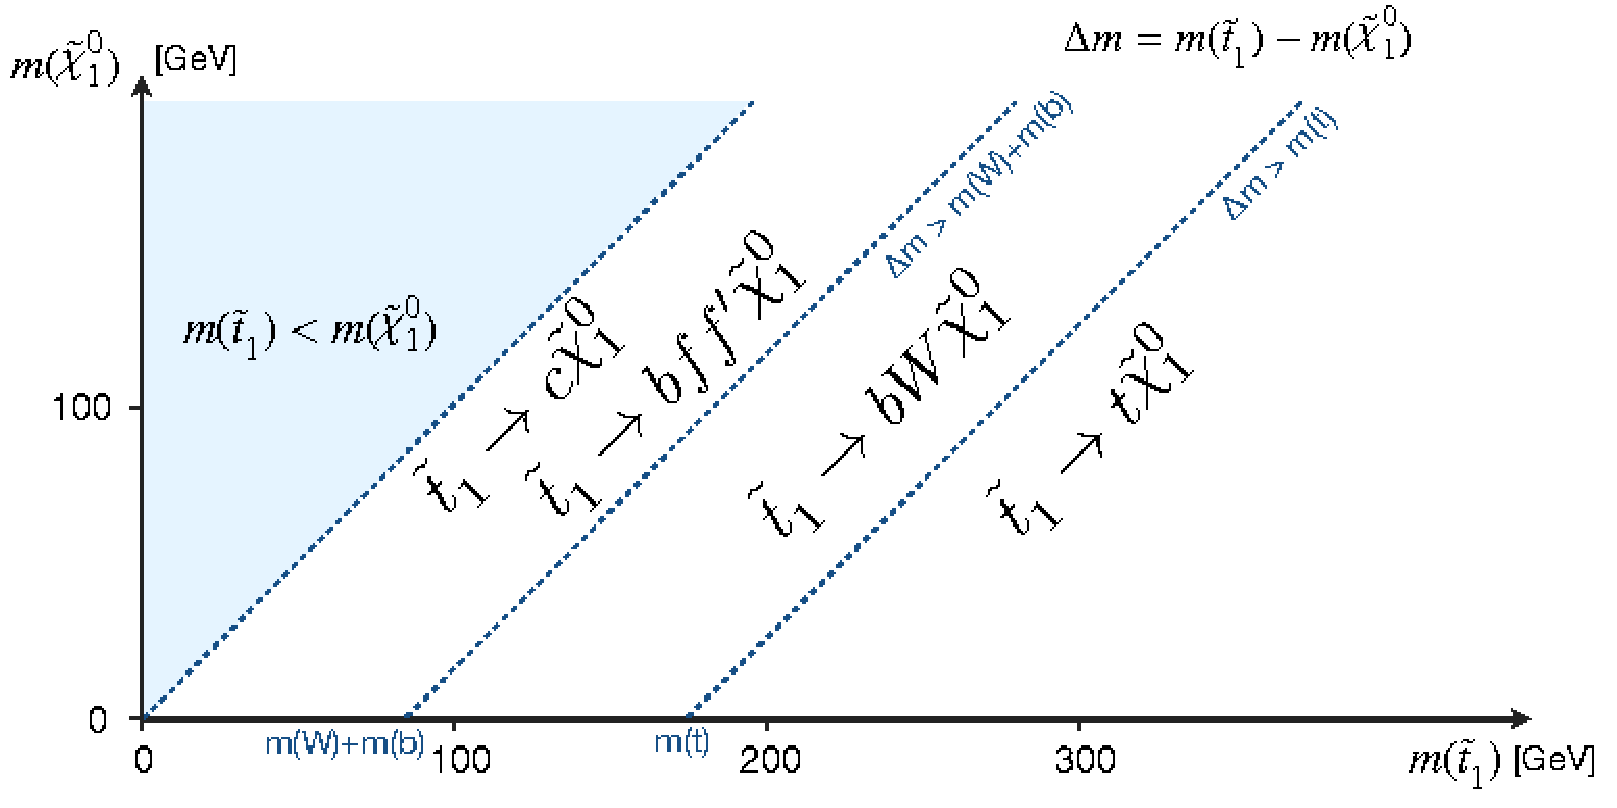
\includegraphics[width=0.75\textwidth]{topSquark_mass_decayModes.pdf}
 	\caption[Top Squark Decay Modes]{Mass parameter space for different decay modes of the top squark.}
 	\label{StopParameterSpace} 
\end{figure}

\begin{table}[!ht]
\begin{center}
\caption[High $\Delta$m Search Regions]{\label{tab:searchregions-hm}Summary of the 130 disjoint search regions that mainly target high \dm~signal models. The high \dm~baseline selection is again $\nj \geq 5$, $\met>250~\GeV$, $\nb\geq1$, and $\dphijonetwothreefour>0.5$.}
\resizebox*{1\textwidth}{!}{

\begin{tabular}{|c|c|c|c|c|c|c|}
	\hline
	\multicolumn{7}{|c|}{$\mtb<175$\,\GeV}  \\
	\hline
	\nj				 & \nb				& \nt			   & \nw				 & \nrt				& \Ht ~[\GeV]		   & \met~[\GeV] 		\\
	\hline
	$\geq7$		& $1, \geq2$  & $\geq0$		 & $\geq0$			& $\geq1$	  & $\geq300$			& $250-300$, $300-400$, $400-500$, $\geq500$ \\
	\hline
	\multicolumn{7}{|c|}{$\mtb\geq175$\,\GeV}  \\
	\hline
	\nj				 & \nb				& \nt			   & \nw				 & \nrt				& \Ht ~[\GeV]		   & \met~[\GeV] 		\\
	\hline
	$\geq5$		& $1,\geq2$   &	$0$				& $0$				   & $0$			 & $\geq1000$		 & $250-350$, $350-450$, $450-550$, $\geq550$ \\
	\hline
	\multirow{6}{*}{$\geq5$} & \multirow{6}{*}{$1$} & $\geq1$ & $0$ & $0$ & $300-1000$, $1000-1500$, $\geq1500$ & $250-550$, $550-650$, $\geq650$\\
						  &					   & $0$			 & $\geq1$			& $0$			  & $300-1300$, $\geq1300$ & $250-350$, $350-450$, $\geq450$ \\
						  &					   & $0$			 & $0$				    & $\geq1$	  & $300-1000$, $1000-1500$, $\geq1500$ & $250-350$, $350-450$, $450-550$, $550-650$, $\geq650$ \\
						  &					   & $\geq1$	 & $\geq1$			& $0$			  & $\geq300$ 			& $250-550$, $\geq550$ \\
						  &					   & $\geq1$	 & $0$					& $\geq1$	  & $\geq300$			& $250-550$, $\geq550$ \\
						  &					   & $0$			 & $\geq1$			& $\geq1$	  & $\geq300$			& $250-550$, $\geq550$ \\
	\hline
	\multirow{10}{*}{$\geq5$} & \multirow{10}{*}{$2$} & $1$ & $0$ & $0$ & $300-1000$, $1000-1500$, $\geq1500$ & $250-550$, $550-650$, $\geq650$\\
						  &					   & $0$			 & $1$					& $0$			& $300-1300$, $\geq1300$ & $250-350$, $350-450$, $\geq450$ \\
						  &					   & $0$			 & $0$				    & $1$	  		& $300-1000$, $1000-1500$, $\geq1500$ & $250-350$, $350-450$, $450-550$, $550-650$, $\geq650$ \\
						  &					   & $1$	 		 & $1$					& $0$			& $\geq300$ 						& $250-550$, $\geq550$ \\
						  &					   & $1$	 		 & $0$					& $1$	  		& $300-1300$, $\geq1300$ & $250-350$, $350-450$, $\geq450$ \\
						  &					   & $0$			 & $1$					& $1$	  		& $\geq300$							& $250-550$, $\geq550$ \\
						  &					   & $2$	 		 & $0$					& $0$			& $\geq300$ 						& $250-450$, $\geq450$ \\
						  &					   & $0$	 		 & $2$					& $0$	  		& $\geq300$ 						& $\geq250$ \\
						  &					   & $0$			 & $0$					& $2$	  		& $300-1300$, $\geq1300$ & $250-450$, $\geq450$ \\
						  &					   & \multicolumn{3}{|c|}{$\nt+\nw+\nrt\geq3$} & $\geq300$ 					   & $\geq250$ \\
	\hline
	\multirow{10}{*}{$\geq5$} & \multirow{10}{*}{$\geq3$} & $1$ & $0$ & $0$ & $300-1000$, $1000-1500$, $\geq1500$ & $250-350$, $350-550$, $\geq550$\\
						  &					   & $0$			 & $1$					& $0$			& $\geq300$ 						& $250-350$, $350-550$, $\geq550$\\
						  &					   & $0$			 & $0$				    & $1$	  		& $300-1000$, $1000-1500$, $\geq1500$ & $250-350$, $350-550$, $\geq550$\\
						  &					   & $1$	 		 & $1$					& $0$			& $\geq300$ 						& $\geq250$ \\
						  &					   & $1$	 		 & $0$					& $1$	  		& $\geq300$ 						& $250-350$, $\geq350$ \\
						  &					   & $0$			 & $1$					& $1$	  		& $\geq300$							& $\geq250$ \\
						  &					   & $2$	 		 & $0$					& $0$			& $\geq300$ 						& $\geq250$ \\
						  &					   & $0$	 		 & $2$					& $0$	  		& $\geq300$ 						& $\geq250$ \\
						  &					   & $0$			 & $0$					& $2$	  		& $\geq300$ 					   & $250-350$, $\geq350$ \\
						  &					   & \multicolumn{3}{|c|}{$\nt+\nw+\nrt\geq3$} & $\geq300$ 					   & $\geq250$ \\
	\hline
\end{tabular}
}
\end{center}
\end{table}

\begin{table}[!ht]
\begin{center}
\caption[Low $\Delta$m Search Regions]{\label{tab:searchregions-lm}Summary of the 53 disjoint search regions that mainly target low \dm~signal models. The low \dm~baseline selection is again $\nj \geq 2$, $\met>250~\GeV$, $\nt=\nw=\nrt=0$, $\nb\geq0$, $\mtb<175~\GeV$ (when applicable), $|\Delta\phi(\text {j}_1,\met)|>0.5, ~~ |\Delta\phi(\text {j}_{2,3},\met)| > 0.15$, $\pt(ISR) > 200$~\GeV, $ |\eta(ISR)| < 2.4$, $|\Delta\phi(j_{\text{ISR}},\met)|>2$, and $\metsig > 10$.}
\resizebox*{1\textwidth}{!}{
\begin{tabular}{|c|c|c|c|c|c|}
	\hline
	$\nj$              & $\nb$                    & $\nsv$             & $\ptisr$~[\GeV]         & $\ptb$~[\GeV]      & $\met$~[\GeV]                           \\
	\hline
	$2-5$              & \multirow{4}{*}{0}       & 0                  & \multirow{4}{*}{$>500$} & \multirow{4}{*}{-} & $450-550$, $550-650$, $650-750$, $>750$ \\
	$\geq6$            &                          & 0                  &                         &                    & $450-550$, $550-650$, $650-750$, $>750$ \\
	$2-5$              &                          & $\geq1$            &                         &                    & $450-550$, $550-650$, $650-750$, $>750$ \\
	$\geq6$            &                          & $\geq1$            &                         &                    & $450-550$, $550-650$, $650-750$, $>750$ \\
	\hline
	\multirow{5}{*}{$\geq2$} & \multirow{5}{*}{1}   & 0                  & $300-500$               & $20-40$            & $300-400$, $400-500$, $500-600$, $>600$ \\
	&                          & 0                  & $300-500$               & $40-70$            & $300-400$, $400-500$, $500-600$, $>600$ \\
	&                          & 0                  & $>500$                  & $20-40$            & $450-550$, $550-650$, $650-750$, $>750$ \\
	&                          & 0                  & $>500$                  & $40-70$            & $450-550$, $550-650$, $650-750$, $>750$ \\
	&                          & $\geq1$            & $>300$                  & $20-40$            & $300-400$, $400-500$, $>500$            \\
	\hline
	$\geq2$            & \multirow{6}{*}{$\geq2$} & \multirow{6}{*}{$\geq0$} & $300-500$               & $40-80$            & $300-400$, $400-500$, $>500$            \\
	$\geq2$            &                          &                          & $300-500$               & $80-140$           & $300-400$, $400-500$, $>500$            \\
	$\geq7$            &                          &                          & $300-500$               & $>140$             & $300-400$, $400-500$, $>500$            \\
	$\geq2$            &                          &                          & $>500$                  & $40-80$            & $450-550$, $550-650$, $>650$            \\
	$\geq2$            &                          &                          & $>500$                  & $80-140$           & $450-550$, $550-650$, $>650$            \\
	$\geq7$            &                          &                          & $>300$                  & $>140$             & $450-550$, $550-650$, $>650$         \\
	\hline
\end{tabular}
}
\end{center}
\end{table}


